\documentclass{article}

% -----------------------------------------------------------------------------
% English Comments Added for Clarity
% This document is a LaTeX file for a homework assignment. The original text is
% in Persian. The comments below are added to explain the structure and packages
% used in the document.
% -----------------------------------------------------------------------------

% --- Package Loading ---
% The following section loads the necessary LaTeX packages for this document.

% The 'neurips' style file is used for formatting.
\usepackage[final]{neurips}

% 'multicol' allows for text to be set in multiple columns.
\usepackage{multicol}

% 'float' provides improved control over floating objects like figures and tables.
\usepackage{float}

% 'caption' is used for customizing the captions of figures and tables.
\usepackage[center]{caption}

% 'inputenc' with the [utf8] option allows for UTF-8 encoded text to be used directly.
\usepackage[utf8]{inputenc}

% 'fontenc' with the [T1] option specifies the font encoding.
\usepackage[T1]{fontenc}

% 'hyperref' creates hyperlinks within the document.
\usepackage{hyperref}

% 'url' provides a simple way to format URLs.
\usepackage{url}

% 'booktabs' is used for creating professional-quality tables.
\usepackage{booktabs}

% 'amsfonts' provides access to blackboard bold math symbols.
\usepackage{amsfonts}

% 'nicefrac' allows for the typesetting of compact fractions.
\usepackage{nicefrac}

% 'microtype' improves the typographic quality of the document.
\usepackage{microtype}

% 'graphicx' is used for including images in the document.
\usepackage{graphicx}

% 'amsmath' provides a wide range of environments for typesetting mathematical formulas.
\usepackage{amsmath}

% 'xepersian' is the main package for typesetting Persian text with XeLaTeX.
\usepackage{xepersian}

% 'kbordermatrix' is used for creating matrices with labels on the borders.
\usepackage{kbordermatrix}

% --- Font Setup ---
% Sets the main text font to "XB Yas.ttf", a Persian font included in the repository.
\settextfont{XB Yas.ttf}

% --- Document Title (in Persian) ---
% The title of the document is "Second Homework".
\title{تمرین دوم}


% The \author macro works with any number of authors. There are two commands
% used to separate the names and addresses of multiple authors: \And and \AND.
%
% Using \And between authors leaves it to LaTeX to determine where to break the
% lines. Using \AND forces a line break at that point. So, if LaTeX puts 3 of 4
% authors names on the first line, and the last on the second line, try using
% \AND instead of \And before the third author name.

\author{%
  امیرحسین مهدی‌نژاد\\
  شماره دانشجویی 810800058\\
  \texttt{mahdinejad@ut.ac.ir} \\
  % examples of more authors
  % \And
  % Coauthor \\
  % Affiliation \\
  % \texttt{email} \\
  % \AND
  % Coauthor \\
  % Affiliation \\
  % Address \\
  % \texttt{email} \\
}

% create title (includes both anonymized and non-anonymized versions)
% \providecommand{\@makepertitle}{}
% \newcommand{\makepertitle}{%
%   \vbox{%
%     \hsize\textwidth
%     \linewidth\hsize
%     \vskip 0.1in
%     \toptitlebar
%     \centering
%     {\LARGE\bf \@title\par}
%     \bottomtitlebar
%       \def\And{%
%         \end{tabular}\hfil\linebreak[0]\hfil%
%         \begin{tabular}[t]{c}\bf\rule{\z@}{24\p@}\ignorespaces%
%       }
%       \def\AND{%
%         \end{tabular}\hfil\linebreak[4]\hfil%
%         \begin{tabular}[t]{c}\bf\rule{\z@}{24\p@}\ignorespaces%
%       }
%       \begin{tabular}[t]{c}\bf\rule{\z@}{24\p@}\@author\end{tabular}%
%     \vskip 0.3in \@minus 0.1in
%   }
% }

\begin{document}


\begin{minipage}{0.1\textwidth}% adapt widths of minipages to your needs

\includegraphics[width=1.1cm]{Photos/UT_logo.png}
\end{minipage}%
\hfill%
\begin{minipage}{0.9\textwidth}\raggedleft
دانشکده فنی، دانشگاه تهران\\
الگوریتم‌های گراف و شبکه - 
دی
ماه 1400\\
\end{minipage}
% \end{}


\makepertitle


% \begin{abstract}
%  این بخش از یک پاراگراف تشکیل شده است که توضیحاتی کلی در مورد مساله و راه حل شما ارائه می‌دهد.
% \end{abstract}

\begin{multicols}{2}

% -----------------------------------------------------------------------------
% --- Homework Questions Start Here ---
% The document is organized into sections for each question.
% -----------------------------------------------------------------------------

% --- Question 1 ---
% This section addresses the first question of the assignment.
\section*{سوال اول}

% The graph for Question 1 is shown here.
\begin{figure}[H]
    \center
    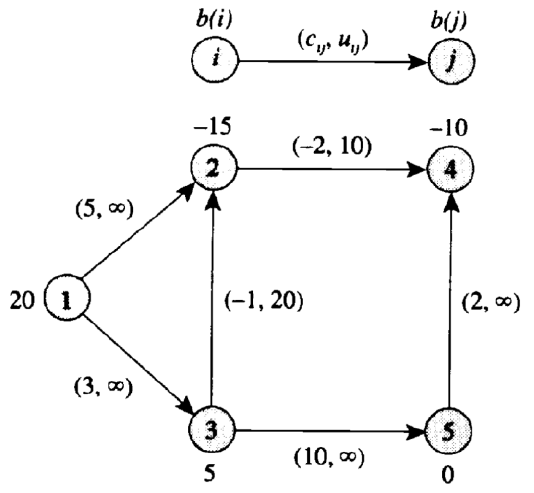
\includegraphics[width=0.9\linewidth]{Photos/HW2/1.png}
    \caption{
    گراف صورت سوال
    }
    \label{fig:my_label}
\end{figure}

% -----------------------------------------------------------------------
% --- Part 1.a: Matrix Representations ---
\subsection*{\lr{1.a}}

% --- Node-Arc Incidence Matrix ---
% This subsection provides the node-arc incidence matrix for the graph.
\subsubsection*{
\lr{node-arc incidence matrix}
}

\renewcommand{\kbldelim}{(}% Left delimiter
\renewcommand{\kbrdelim}{)}% Right delimiter
\[
  \kbordermatrix{
    & e_{12} & e_{13} & e_{24} & e_{32} & e_{35} & e_{54} \\
    1 & 1 & 1 & 0 & 0 & 0 & 0 \\
    2 & -1 & 0 & 1 & -1 & 0 & 0\\
    3 & 0 & -1 & 0 & 1 & 1 & 0 \\
    4 & 0 & 0 & -1 & 0 & 0 & -1 \\
    5 & 0 & 0 & 0 & 0 & -1 & 1
  }
\]

% --- Node-Node Adjacency Matrix ---
% This subsection provides the node-node adjacency matrix for the graph.
\subsubsection*{
\lr{node-node adjacency matrix}
}

\renewcommand{\kbldelim}{(}% Left delimiter
\renewcommand{\kbrdelim}{)}% Right delimiter
\[
  \kbordermatrix{
    & 1 & 2 & 3 & 4 & 5 \\
    1 & 0 & 1 & 1 & 0 & 0 \\
    2 & 0 & 0 & 0 & 1 & 0 \\
    3 & 0 & 1 & 0 & 0 & 1 \\
    4 & 0 & 0 & 0 & 0 & 0 \\
    5 & 0 & 0 & 0 & 1 & 0
  }
\]

% -----------------------------------------------------------------------
% --- Part 1.b: Handling Negative Costs ---
% This subsection describes the process of eliminating negative costs in the graph
% by reversing the direction of arcs.
\subsection*{\lr{1.b}}
\begin{figure}[H]
    \center
    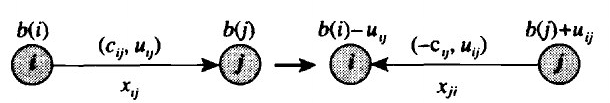
\includegraphics[width=0.99\linewidth]{Photos/HW2/arc_reverse.png}
    \caption{
    روال معکوس کردن جهت یال، برای از بین بردن
    \lr{cost}
    منفی
    }
    \label{fig:my_label}
\end{figure}
اگر ابتدا طبق روال شکل فوق، این کار را برای یال
$(3, 2)$
انجام دهیم، مقادیر به این صورت تغییر خواهند کرد:
$$b(3) = -15, b(2) = 5$$
$$c_{23} = 1, u_{23} = 20$$
سپس همین کار را برای یال
$(2, 4)$
نیز انجام می‌دهیم:
$$b(2) = -5, b(4) = 0$$
$$c_{42} = 2, u_{42} = 10$$

% -----------------------------------------------------------------------
% --- Part 1.c: Eliminating Arc Capacities ---
% This subsection explains how to remove arc capacities by introducing new nodes.
\subsection*{\lr{1.c}}
\begin{figure}[H]
    \center
    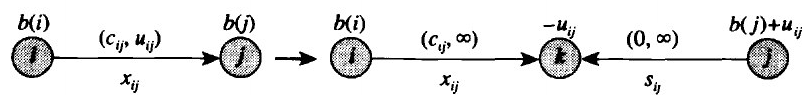
\includegraphics[width=\linewidth]{Photos/HW2/remove_c.png}
    \caption{
    روال از بین بردن ظرفیت یال
    }
    \label{fig:my_label}
\end{figure}
اگر ابتدا طبق روال شکل فوق، این کار را برای یال
$(3, 2)$
انجام دهیم و نود
$6$
را بین آن‌ها اضافه کنیم، خواهیم داشت:
$$b(3) = 5, b(6) = -20, b(2) = 5$$
$$c_{36} = -1, u_{36} = \infty$$
$$c_{26} = 0, u_{26} = \infty$$
سپس همین کار را برای یال
$(2, 4)$
تکرار کرده و نود
$7$
را بین آن‌ها اضافه می‌کنیم:
$$b(2) = 5, b(7) = -10, b(4) = 0$$
$$c_{27} = -2, u_{27} = \infty$$
$$c_{47} = 0, u_{47} = \infty$$

% -----------------------------------------------------------------------
% --- Part 1.d: Handling Non-zero Lower Bounds ---
% This subsection demonstrates how to make all lower bounds zero.
\subsection*{\lr{1.d}}
\begin{figure}[H]
    \center
    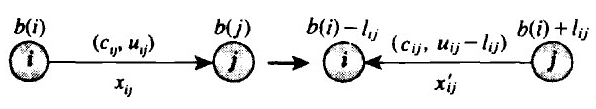
\includegraphics[width=0.9\linewidth]{Photos/HW2/nonzero_lb.png}
    \caption{
    روال صفر کردن
    \lr{lower bound}
    ها
    }
    \label{fig:my_label}
\end{figure}
اگر طبق روال شکل فوق، این کار را برای یال
$(1, 2)$
انجام دهیم خواهیم داشت:
$$b(1) = 15, b(2) = -10$$
$$c_{21} = 5, u_{21} = \infty$$
همچنین برای یال
$(3, 5)$
نیز بدین شکل خواهد شد:
$$b(3) = 0, b(5) = 5$$
$$c_{53} = 10, u_{53} = \infty$$

% -----------------------------------------------------------------------
% --- Part 1.e ---
% This part is noted as being a repeat of part 1.c.
\subsection*{\lr{1.e}}
این بند مشابه بند
\lr{c}
همین سوال تکرار شده است.\\
\rule{\linewidth}{1pt}
% -----------------------------------------------------------------------
% --- Question 2 ---
% This section addresses the second question of the assignment.
\section*{سوال دوم}
% The graph for Question 2 is shown here.
\begin{figure}[H]
    \center
    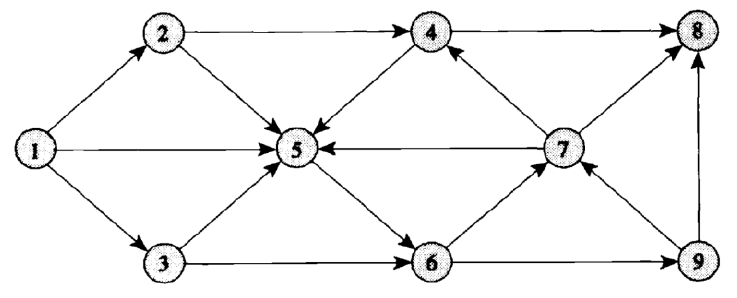
\includegraphics[width=0.9\linewidth]{Photos/HW2/2.png}
    \caption{
    گراف صورت سوال
    }
    \label{fig:my_label}
\end{figure}

% --- Part 2.a: BFS and DFS Trees ---
% This subsection shows the Breadth-First Search (BFS) and Depth-First Search (DFS)
% trees for the given graph.
\subsection*{\lr{2.a}}
\begin{figure}[H]
    \center
    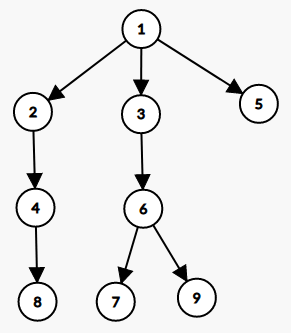
\includegraphics[width=0.45\linewidth]{Photos/HW2/bfs2.png}
    \caption{
    درخت
    \lr{BFS}
    }
    \label{fig:my_label}
\end{figure}

\begin{figure}[H]
    \center
    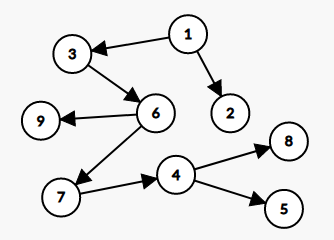
\includegraphics[width=0.5\linewidth]{Photos/HW2/backedge.png}
    \caption{
    درخت
    \lr{DFS}
    }
    \label{fig:my_label}
\end{figure}
% -----------------------------------------------------------------------
% --- Part 2.b: Acyclicity and Topological Sort ---
% This subsection discusses the acyclicity of the graph and provides a
% topological sort.
\subsection*{\lr{2.b}}
گراف صورت سوال
\lr{Acyclic}
نیست و می‌توان دور جهت‌دار
$5 \rightarrow 6 \rightarrow 7 \rightarrow 5$
را برای نقض بدون دور بودن آن مثال زد.\\
با توجه به درخت
\lr{DFS}
بند قبلی می‌توان نتیجه گرفت که یال
$(5, 6)$
که در گراف اصلی وجود دارد، به عنوان
\lr{Back edge}
دیده می‌شود و با حذف آن، گراف دور جهت‌دار نخواهد داشت.

پس از اینکه دورهای گراف را حذف کردیم می‌توان از روش
\lr{BFS}
(الگوریتم کان) به ترتیب
[1,2,3,4,5,6,9,7,8]
رسید و همچنین از روش
\lr{DFS}
به ترتیب
[1,3,2,4,5,6,9,7,8]
می‌رسیم. یعنی ترتیب توپولوژیک آن یکتا نیست.\\
\rule{\linewidth}{1pt}

% -----------------------------------------------------------------------
% --- Question 3: Dijkstra's Algorithm ---
% This section explains and demonstrates Dijkstra's algorithm for finding the
% shortest path in a graph.
\section*{سوال سوم}
% The graph for Question 3 is shown here.
\begin{figure}[H]
    \center
    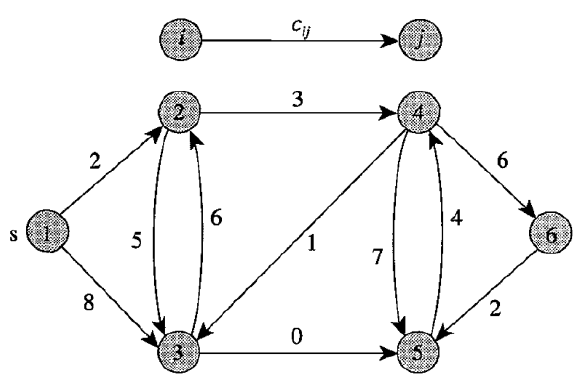
\includegraphics[width=0.75\linewidth]{Photos/HW2/3.png}
    \caption{
    گراف صورت سوال
    }
    \label{fig:my_label}
\end{figure}
در الگوریتم دایجسترا ابتدا
$\text{dist}(1) = 0$
و به ازای هر راس دیگر 
\lr{v}
مقدار
$\text{dist}(v) = \infty$
در نظر گرفته می‌شود.\\
در هر مرحله نزدیک‌ترین راس
مثل \lr{x}
پیدا شده و فاصله‌ی دیگر رئوس با توجه به فاصله‌ی آن آپدیت می‌شود:
$$\text{dist}(v) = min(\text{dist}(v), \text{dist}(x) + \text{w}(x, v))$$
به ازای هر راس این پروسه تکرار می‌شود و مجموعه‌ی همسایه‌های آن بررسی می‌شود. در هر دور از این الگوریتم، راسی که کوتاه‌ترین فاصله با
\lr{s}
را دارد به مجموعه‌ی نهایی افزوده می‌شود، چرا که کوتاه‌ترین مسیر این راس از یکی از رئوس مجموعه می‌گذرد که در مراحل قبلی فاصله‌ی آن‌ها بدست آمده و توسط رئوس دیگر بروز شده است.
% The result of running Dijkstra's algorithm is shown in the figure below.
\begin{figure}[H]
    \center
    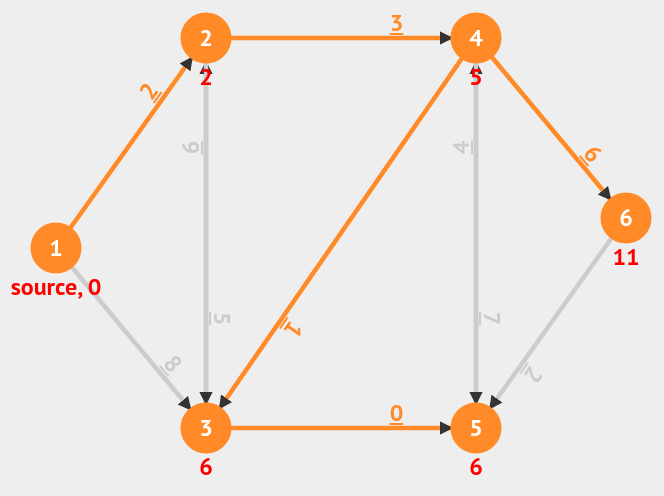
\includegraphics[width=0.9\linewidth]{Photos/HW2/dijk.png}
    \caption{
    نتیجه‌ی اجرای الگوریتم دایجسترا با شروع از راس شماره یک
    }
    \label{fig:my_label}
\end{figure}

\end{multicols}
\end{document}
